\chapter{Example Model of Packet Processing System}
\label{chapter:example-simulation-model}
In this chapter, we present an example simulation model of Cavium OCTEON II CN6880 network processing unit~\cite{Cavium OCTEON}.

\todo[inline]{We will first demonstrate the measurement hardware and the setup needed to obtain the reference values for the simulation model. Two different measurements will be done, one to measure the communication latencies and another to measure the memory latencies. After that, we will plug in the reference values to the model and describe the relevant details of it.}

\section{Cavium OCTEON II CN6880}
\label{sec:cavium-octeon}

Cavium Octeon II CN6880 is a 32 MIPS core network processing unit, optimized for high-performance, high-bandwidth, and low power consumption software-defined control-plane~\cite{control-plane} and data-plane~\cite{data-plane} applications.

CN6880 provides several hardware acceleration units for enhanced packet processing and minimized software development complexity. The packet management accelerators offload the actual packet processing cores from many general packet receive, buffering, buffer management, flow classification, quality of service, and transmit processing. The accelerator functions can be customized using software, and accessing the configuration registers.~\cite{cavium:2010:fundamentals}

The packet input processor unit (PKI) and input packet data unit (IPD) work together to manage the received packets, and to perform needed processing before scheduling the packets to application cores. They automatically handle most of the processing requirements of the layer 2 to layer 7 open systems interconnection model~\cite{OSI model}. Once the required computation is done, the PKI unit sends the packet's work entry to the SSO unit to be scheduled for processing.~\cite{cavium:2010:fundamentals}

The packet transmission is handled by the packet transmission unit (PKO). When a core finishes a packet processing, it notifies the PKO that the packet is ready for transmission. The PKO then directly copies the packet data from the shared memory into its internal memory, optionally computes checksums for the packet header, transmits the packet, and optionally frees the packet data from the memory.~\cite{cavium:2010:fundamentals}

One of the key features of the CN6880 is its scheduling/synchronization and order unit (SSO). It frees the actual packet processing applications, running on the 32 MIPS cores, from the complex packet scheduling and ordering tasks. The cores execute a loop, and when a core is ready for the next packet, it requests work from the SSO, which then schedules the next work based on the quality of service priority and work group.~\cite{cavium:2010:fundamentals}

The SSO also provides efficient locking mechanisms for protecting the critical regions without explicit software locking, and allows packet processing to be done in parallel or atomically, while still maintaining the packet flow order. The processing cores can also be dedicated for specific flows. One of our goals is to be able to model the scheduling functionality with PSE, as it is crucial to the packet latency and throughput when processing several flows at the time.~\cite{cavium:2010:fundamentals}

The memory latencies have large effect in the packet processing times. The CN6880 provides several memory policies for optimized multi-core packet processing. Each of the 32 cores have dedicated L1 data and instruction cache, and a shared L2 cache. The L1 data cache provides a hybrid write-through, write-back policy, using a write buffer mechanism, and the L2 cache implements a write-back policy. Several other cache related features are offered, for example to avoid unnecessary data writes after the packet transmission, and to automatically send the received packet header to L2 cache and the packet data to main memory, bypassing the L2 cache.~\cite{cavium:2010:fundamentals}

\section{Simulation Model}
\label{sec:simulation-model}

We created a simulation model of the Cavium OCTEON II CN6880 network processing unit with Performance Simulation Environment. The model is a high level abstraction of the real unit. As our interests are mainly in the applications' effect on the packet throughput and latency, we will not model the specific details of the hardware components. Figure \ref{fig:full-model} shows a layered representation of the main components of the model: workload, hardware, and software.

\begin{figure}[h]
  \begin{center}
    %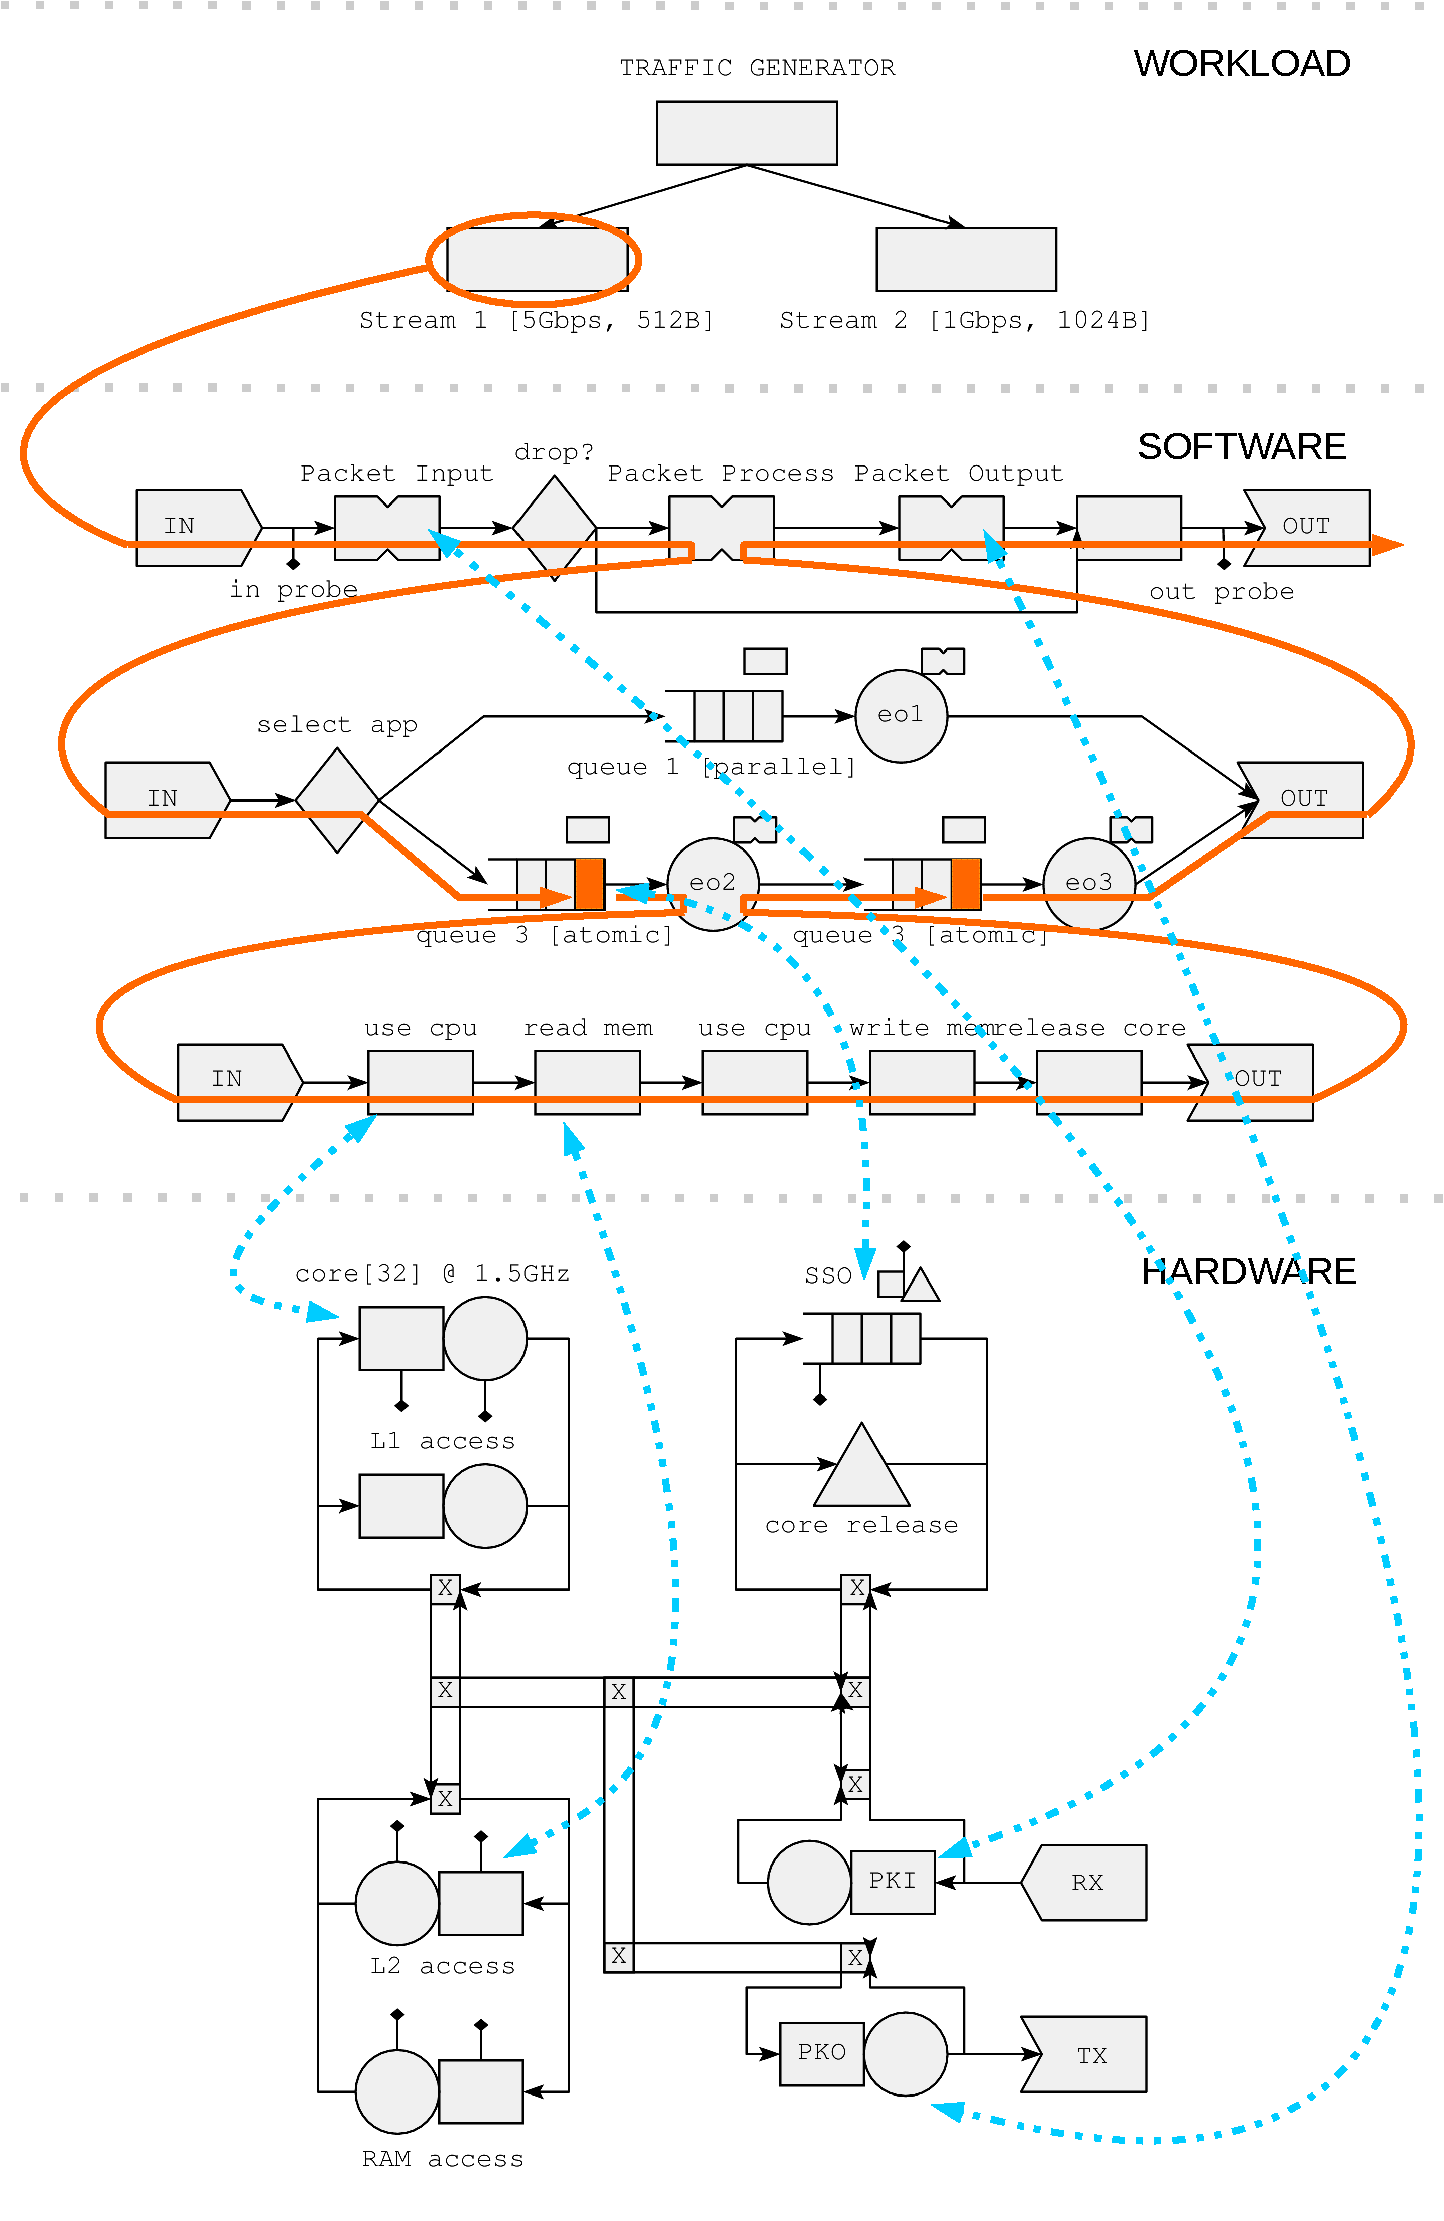
\includegraphics[width=\textwidth]{images/fullmodel-crop.pdf}
    \caption{Graphical presentation of the OCTEON II CN6880 PSE model. The workload model (top) generates network packets, which then flow through the software model, consuming the hardware resources. The orange arrows represent an example of a packet's path through the software model, and the blue arrows the resource usage at each software model node.}
    \label{fig:full-model}
  \end{center}
\end{figure}

The workload model, at the top of the picture, consists of two packet streams. The TRAFFIC GENERATOR node has a lifetime of 0.5 seconds, and it triggers the streams with interval drawn from a uniform distribution with parameters 0.00005 and 0.00015. The streams have lifetime of 0.0004 seconds, and interval drawn from a lognormal distribution. The packet sizes of the streams are defined with the size attribute. Both of the streams also specify an appId attribute that is used to define the processing application in the software model. The packets from both streams enter the IN node of the top level software model.

The software model is divided into several submodels. The top level model consists of packet input, packet processing and packet output submodels. The submodel view of the packet input and packet output are omitted from the picture for the sake of simplicity. In both of these phases, the core and memory usage is linearly dependent on the packet size. In the input phase, the packet consumes specific amount of core cycles for the header processing, and copies the packet header and the packet data to the memory. Packet output node copies the packet from the memory, and consumes certain amount of clock cycles for the packet checksum calculations.

The packet processing submodel is presented in the middle software layer. The select app node forwards each of the packets to one of the two packet processing application, based on the appId attribute defined in the workload model. The queue nodes represent the core scheduling done by the SSO hardware unit. The packets arriving in the upper application have priority of 1, and they can be processed in parallel. In the application below, there are 2 atomic queues with priority 3. When the packet receives the passive resource from SSO, it can enter the execution object (eo). The execution objects are submodels that consume core cycles and memory similarly to the packet input and packet output submodels presented above.

The hardware model is a simple one level model containing no submodels. In the bottom left hand corner, there are PKI and PKO devices providing processor cycles for the packet input and packet output phases. The only passive resource node, SSO, provides core access resources, that can be released with the core release node. The application cores are shown in the top left corner of the hardware layer. There are 32 cores, and a specific L1 cache access for each of them. The L2 and RAM memory resources provide the delay for reading and writing to memory.

The probes, attached to the SSO unit, the cores, and the memory nodes, are used to gather statistics from the execution. Each of the units have two probes, one that measures the resource usage, and other that measures the queue for the corresponding resource. In this hardware model, the routing nodes (squares) and the edges connecting the resources do not have any functional meaning, but are used solely to mimic the graphical models of the unit presented in~\cite{cavium:2010:fundamentals}.

\section{Characteristic Measurements}
\label{sec:characteristic-measurements}

For the model to represent the packet latencies and throughput with enough accuracy, the model needs to be filled with apposite entity parameters. Some of model parameters are simple enough to be obtained directly from~\cite{cavium:2010:fundamentals}, while others are either unavailable, or are presented in a form unsuitable for our simulation model. The missing parameters are obtained by conducting measurements on the real CN6880 hardware.

% We believe that, by determining the latecies of input phase and output phase, the behaviour of memory, and modeling the packet scheduler with enough accuracy, the sought applications' effects to the packet latencies and throughput come up with enough accuracy.

% For our approach to be valid, i.e. the abstraction of the communication latencies to be precise enough, we have to assume the fastpath is not the bottleneck in the processing phase. This assumption is reasonable because ...

% \fixme{
%   TODO:
%   \begin{itemize}
%   \item because the fastpath hardware is optimized for this task
%   \item find reference
%   \item maybe justify the stuff with some kind of rough back-of-the-envelope calculation?
%   \end{itemize}
% }

\subsection{Communication Latencies}

The input and output phase latencies are measured by generating traffic from external machine, and passing it through two CN6880 units back to the generator itself. The measurements were done at two independent points in the processing path, to validate the accuracy of the measurements.

\begin{figure}[ht]
  \begin{center}
    \tikzstyle{block} = [draw, rectangle, thick, minimum height=2em, minimum width=2em]
\tikzstyle{dot} = [circle, inner sep=0pt, minimum size=1mm, fill=black,draw=black]
\tikzstyle{connector} = [->, thick]
\tikzstyle{line} = [thick]

\begin{tikzpicture}
  \small
  % node placement with matrix library: 5x4 array
  \matrix[ampersand replacement=\&, row sep=0.2cm, column sep=0.4cm] {
    \node[block] (l1) {External Traffic-Generator}; \& \& \&
    \node[block] (c1) {Forward Blade}; \& \& \&
    \node[block] (r1) {Swap Blade}; \& \\
  };

  %% Traffic gen probes
  \node [dot] (ld1) at ($(l1.10) + (0cm, 0.4cm)$) {};
  \draw [line] (l1.10) -- node[] {} (ld1);

  \node [dot] (ld2) at ($(l1.-10) + (0cm, -0.4cm)$) {};
  \draw [line] (l1.-10) -- node[] {} (ld2);

  %% Forward blade probes
  \node [dot] (cd1) at ($(c1.18) + (0cm, 0.4cm)$) {};
  \draw [line] (c1.18) -- node[] {} (cd1);

  \node [dot] (cd2) at ($(c1.-18) + (0cm, -0.4cm)$) {};
  \draw [line] (c1.-18) -- node[] {} (cd2);

  %% Swap blade probes
  \node [dot] (rd1) at ($(r1.157) + (0cm, 0.4cm)$) {};
  \draw [line] (r1.157) -- node[] {} (rd1);

  \node [dot] (rd2) at ($(r1.-157) + (0cm, -0.4cm)$) {};
  \draw [line] (r1.-157) -- node[] {} (rd2);

  %% Arrows connecting the nodes

  \draw [connector] (l1.7) -- node[] {} (c1.168);
  \draw [connector] (c1.12) -- node[] {} (r1.166);
  \draw [connector] (r1.-166) -- node[] {} (c1.-12);
  \draw [connector] (c1.-168) -- node[] {} (l1.-7);

\end{tikzpicture}

%%% Local Variables:
%%% mode: latex
%%% TeX-master: "../thesis-hartikainen.tex"
%%% End:

    \caption{The setup used to measure the communication latencies. The measurement points shown with the probes.}
    \label{fig:comm-setup}
  \end{center}
\end{figure}
\todo[inline]{Make figure \ref{fig:comm-setup} clearer, Emphasize the input and output parts of the flow.}

In figure~\ref{fig:comm-setup}, the rectangles represent three different computing units (traffic generator, forward unit, and swap unit), and the probes present the points of time measurements. The traffic generator is a typical desktop computer running Linux operating system, and the traffic was generated by Mausezahn~\cite{mausezahn}. Both of the CN6880 units are running Linux operating systems.

The packet is first generated at the packet generator and sent to the forward unit at time $t_{d0}$. Forwarding unit receives the packet, does the needed processing and forwards the packet to the swap unit at time $t_{d1}$. The swap unit receives the packet at time $t_{r2}$, does the same processing as the forward unit (except with different destination address), and forwards the packet back to the forward unit at time $t_{d2}$. Finally the forward unit receives the packet at time $t_{r1}$ and forwards it to the traffic generator, which marks it received at time $t_{r0}$. The time $t_{f}$ spent in the input and output phase of one unit is then

\begin{equation}
  \label{eq:1}
  t_{f} = \frac{t_{r1} - t_{d1} - (t_{d2} - t_{r2})}{2}.
\end{equation}

We measured the times for packet sizes of 64B, 128B, 256B, 512B, 1024B, and 1500B, repeating the measurement for each packet 10000 times. Figure~\ref{fig:comm-latency} shows the resulting times $t_{f}$ for the different packet sizes.

\begin{figure}[h]
  \begin{center}
    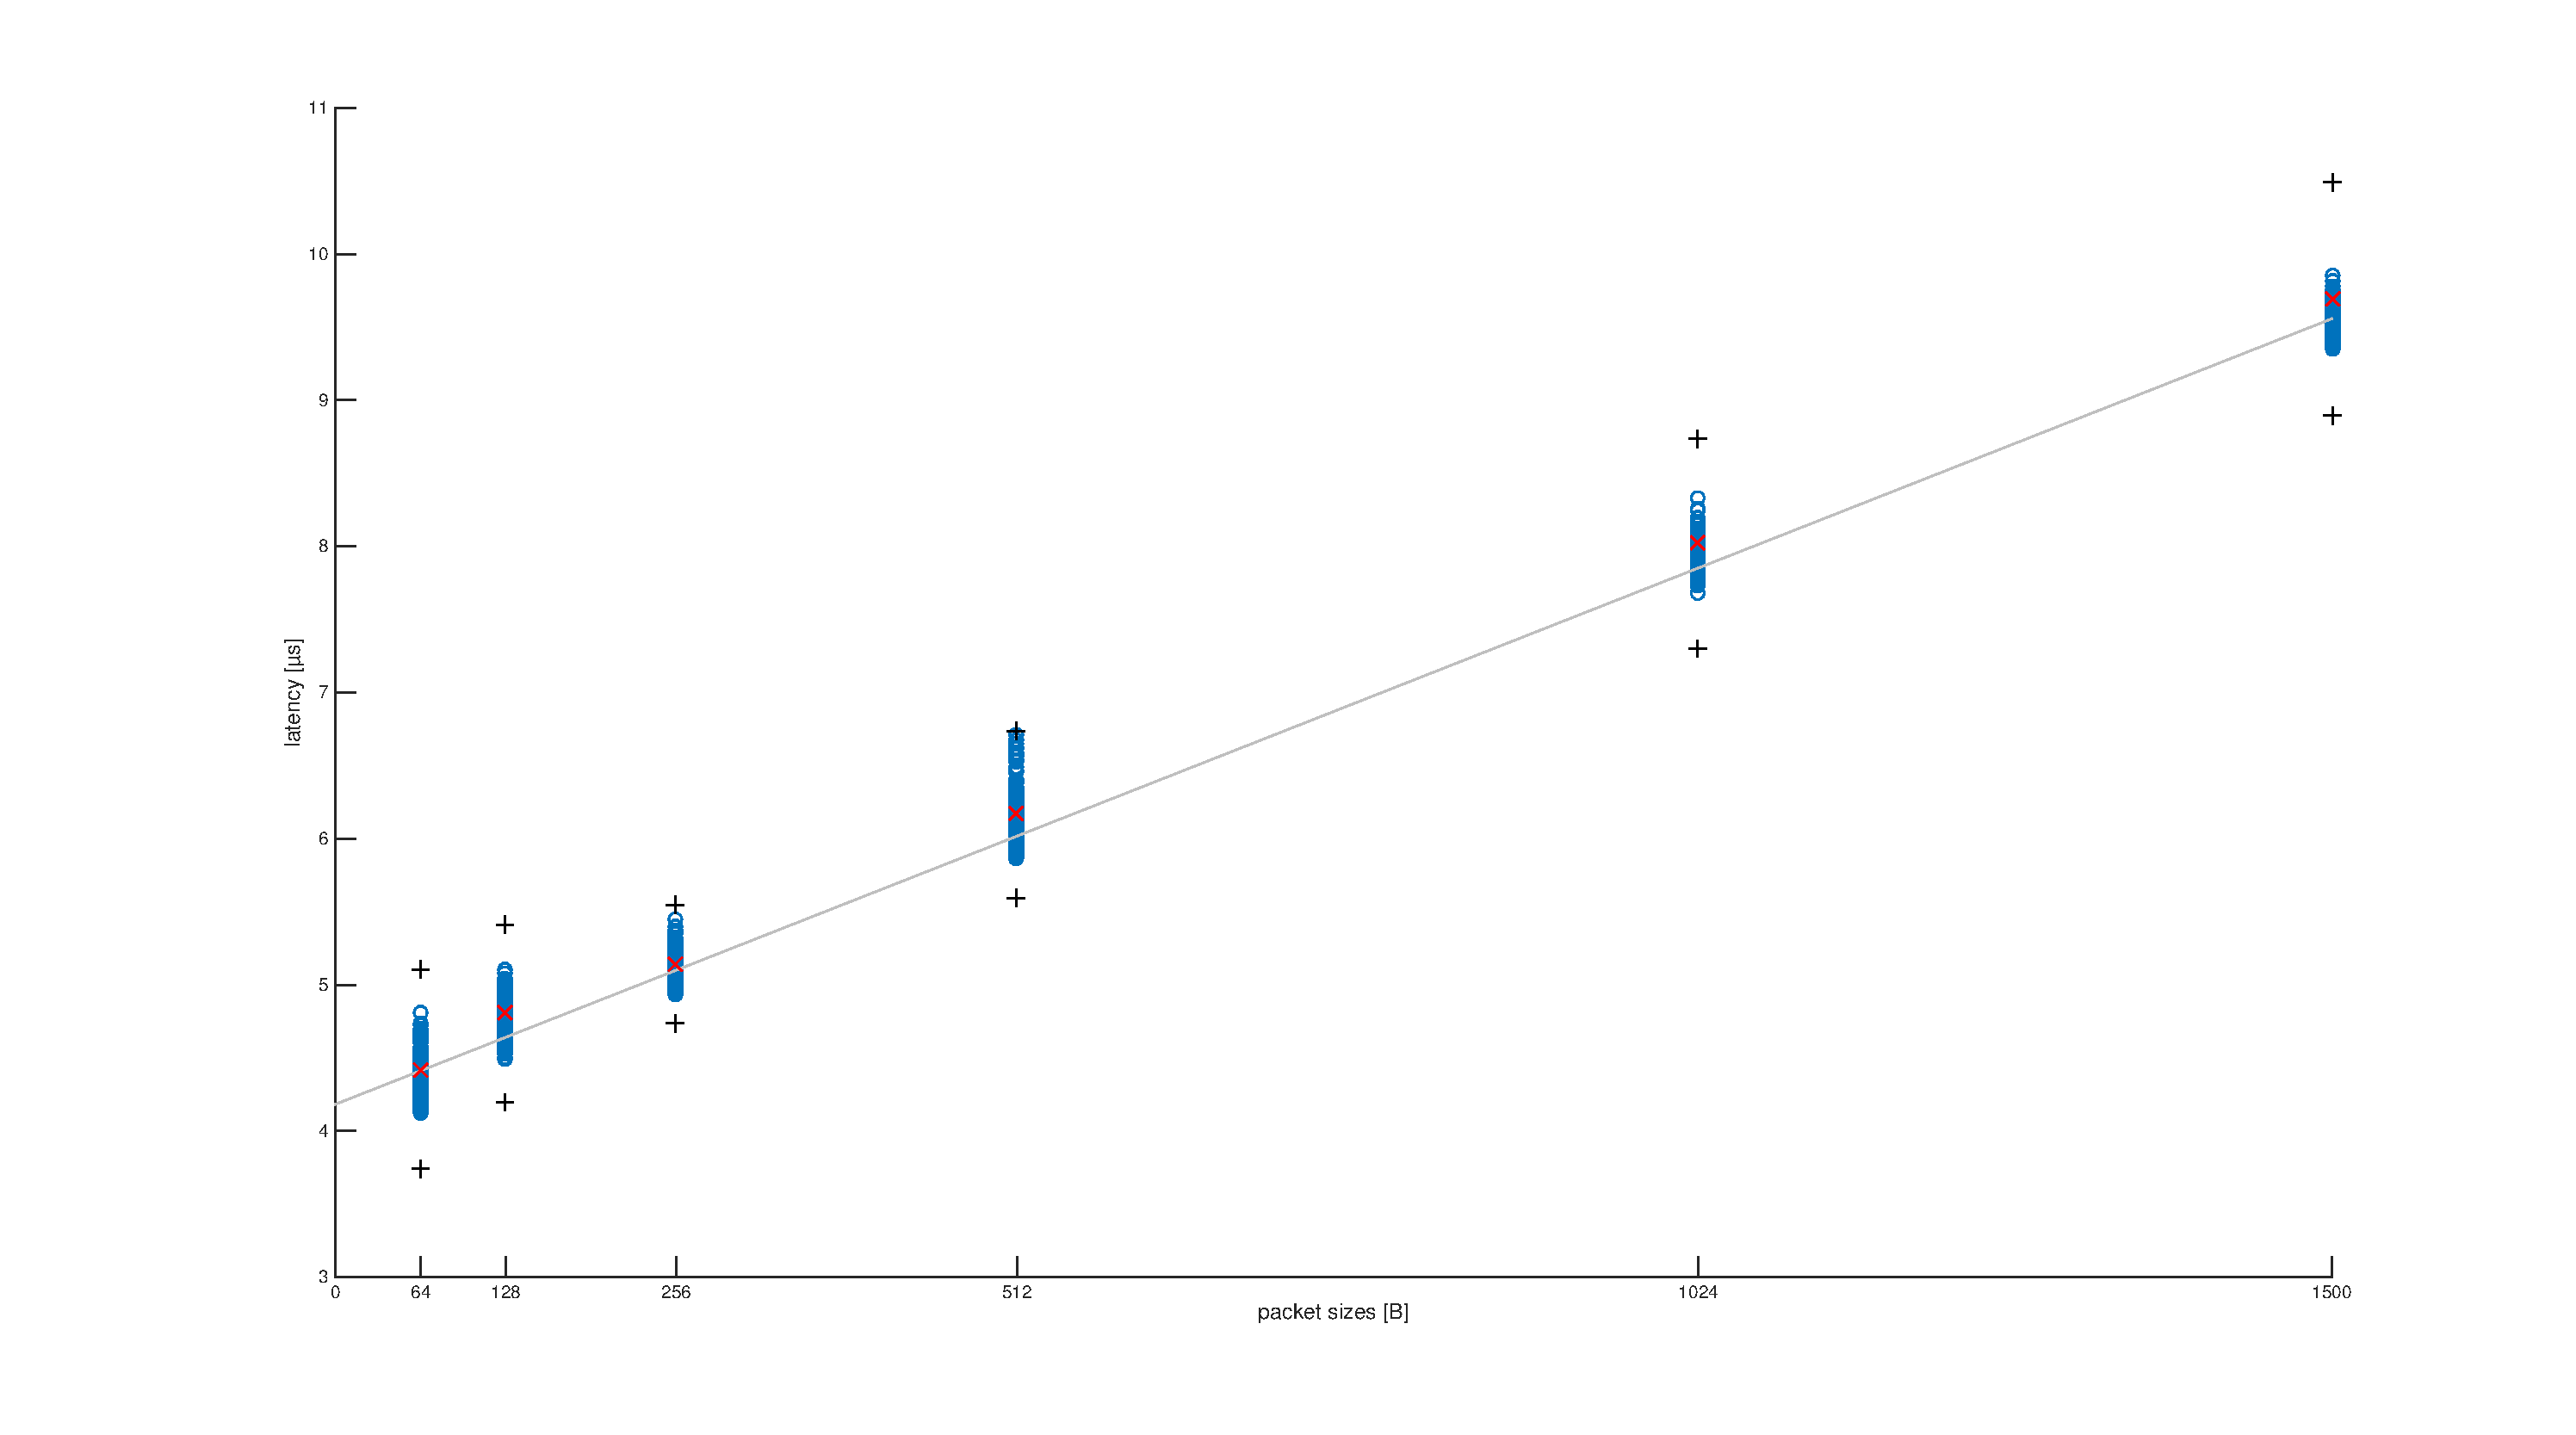
\includegraphics[width=\textwidth]{images/comm-latency.pdf}
    \caption{Latency of the input and output phase of the CN6880 unit. Averages shown marked as red x, and the 99\% confidence intervals with +. The trendline is of equation.}
    \label{fig:comm-latency}
  \end{center}
\end{figure}
\todo[inline]{check the confint}
\todo[inline]{latency = a*packetsize + constant}

As shown in the Figure ~\ref{fig:comm-latency}, the time spent in the input and output phase of the unit is linear regarding to the packet size. The variation of the data is relatively small, and all the measurements correspond to the values measured with the external traffic-generator.

\todo[inline]{the following needs to be explained somewhere with the other fastpath stuff.}
\todo[inline]{Regardless of the packet size, the size of the work queue entry handled by the input/output units is the same.}
\todo[inline]{Also, the forward/swap code is constant in terms of packet size.}
\todo[inline]{Only operation that is dependent on the packet size is the copy from input to L2/RAM and from L2/RAM to output unit.}

As explained earlier\todo{actually explain this}, the only packet size dependent operations in the input/output phase are the  memory transfers between the memory (L2/RAM) and PKI or PKO.

\subsection{Memory Delays}

Memory delays were measured using Multi-core Processor Architecture and Communication (MPAC) benchmarking library. \ref{referenssi} Both, latency and throughput, were measured using for different dataset sizes and number of threads.

\begin{figure}[h]
  \begin{center}
    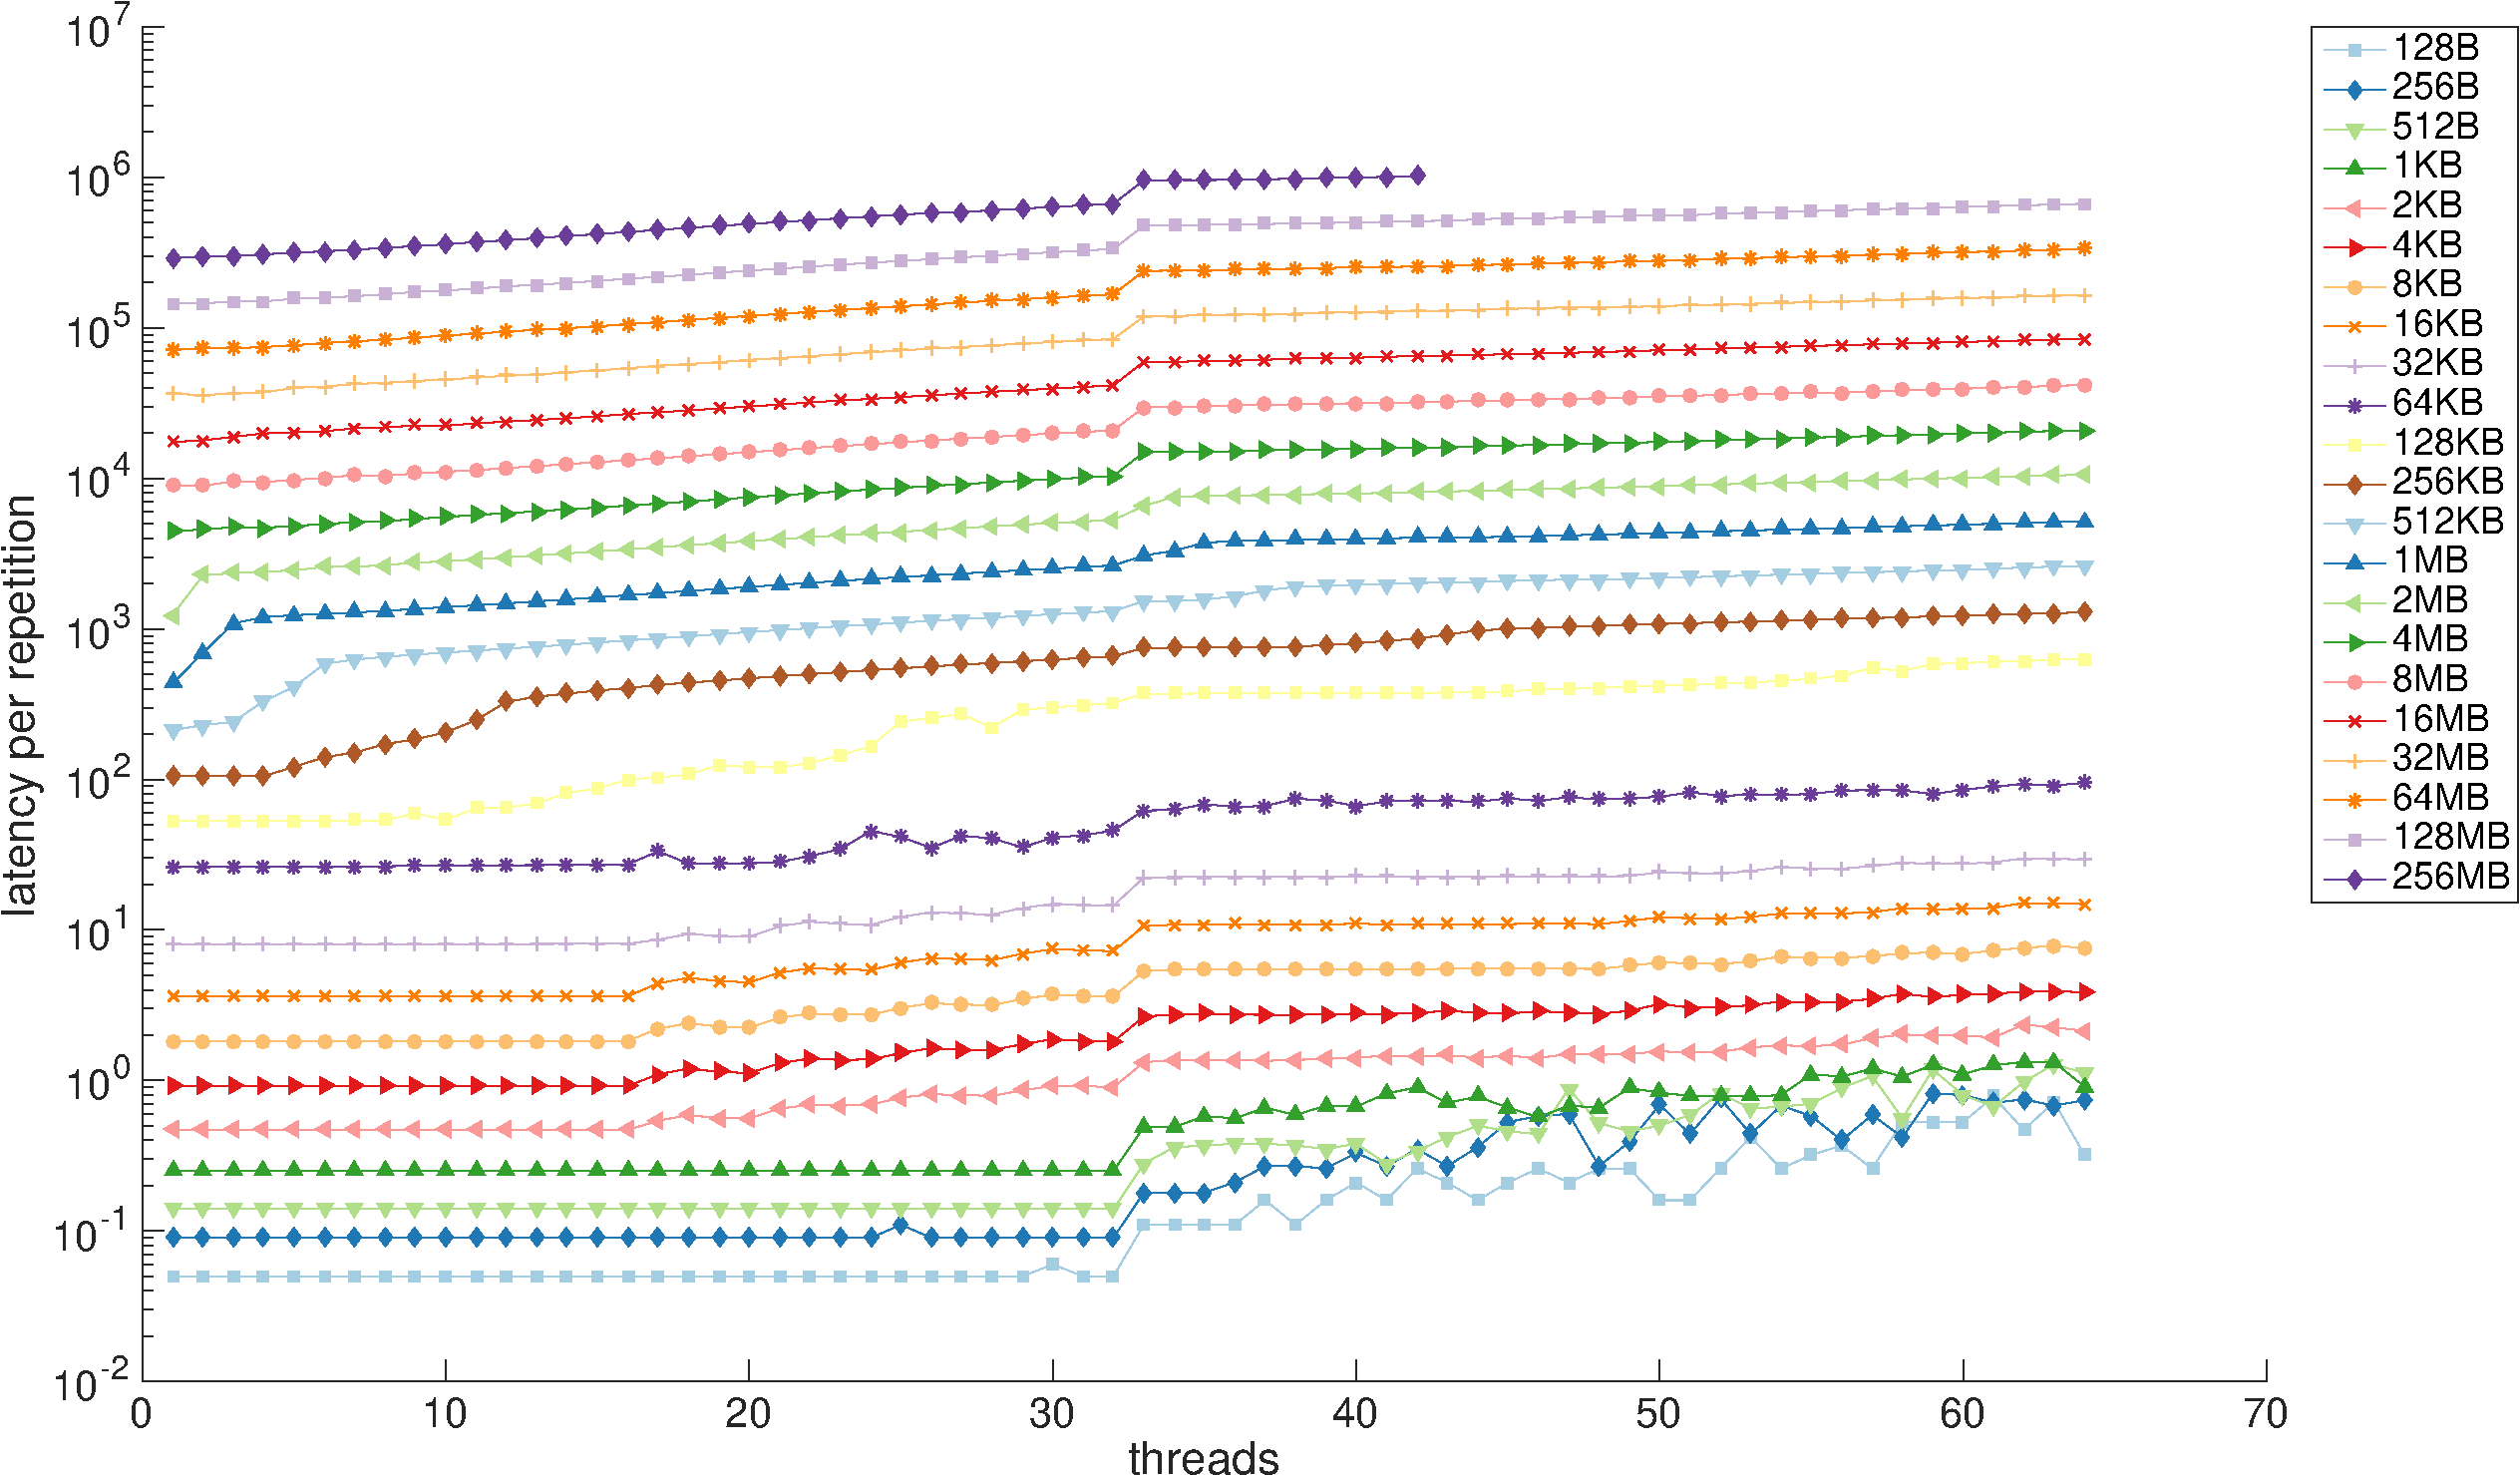
\includegraphics[width=\textwidth]{images/mem-latency.pdf}
    \caption{Memory latencies of the example NPU, measure by MPAC.}
    \label{fig:mem-latency}
  \end{center}
\end{figure}

\todo[inline]{logarithmic Y-scale}
\todo[inline]{explain the figure}

\begin{figure}[h]
  \begin{center}
    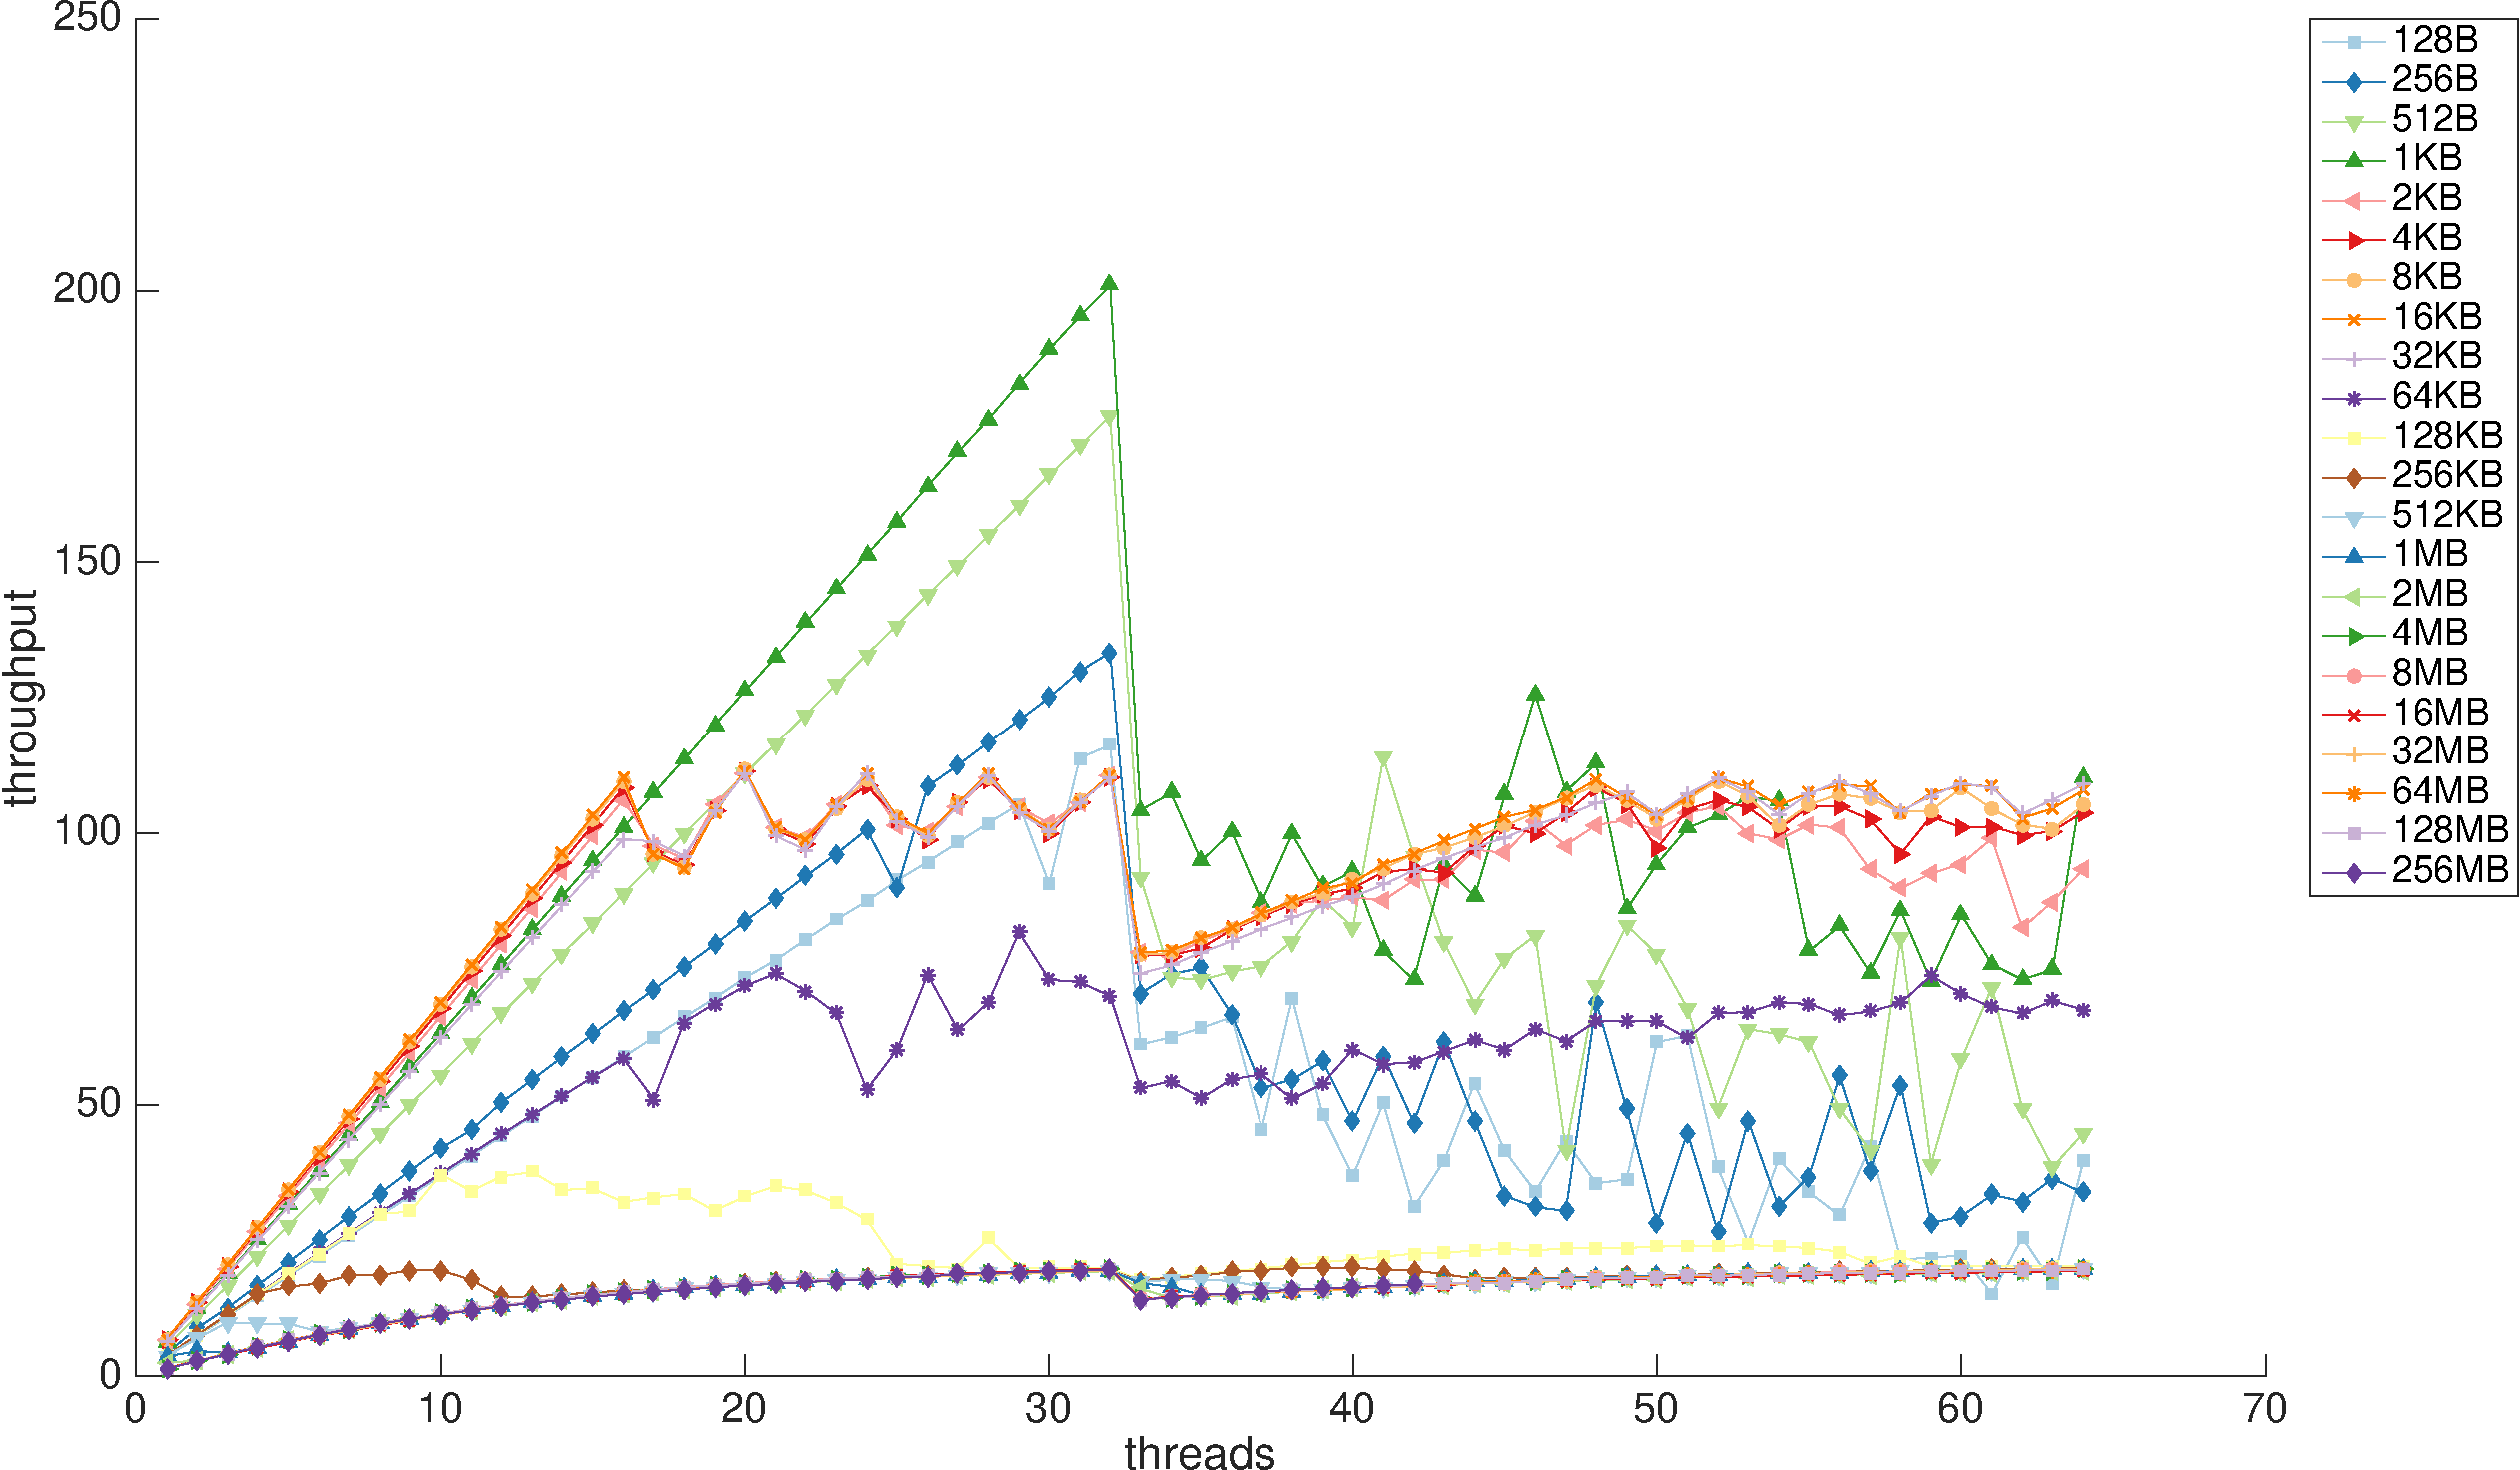
\includegraphics[width=\textwidth]{images/mem-throughput.pdf}
    \caption{Memory throughput of the example NPU, measure by MPAC.}
    \label{fig:mem-throughput}
  \end{center}
\end{figure}

\todo[inline]{explain the figure}

\section{Workload Model}
\todo[inline]{ workload }


\section{Hardware Model}
\todo[inline]{ Scheduler, input/output, NPU nodes }


\section{Software Model}
\todo[inline]{ Scheduler, OpenEM-type application model }

%%% Local Variables:
%%% mode: latex
%%% TeX-master: "thesis-hartikainen"
%%% End:
